
\chapter{Getting started}

	\begin{onehalfspace}

		\section{System requirements}

			%SPAMDA has been developed in Java, therefore it is a multi-platform software tool. In this way, any computer able to install and run a Java Virtual Machine (JVM) will be enough for running the developed tool.
			
			SPAMDA has been developed in Java, therefore it is a multi-platform software tool. In this way, any computer having Java Virtual Machine (JVM) installed would be able to run the developed tool.
			
			As SPAMDA has been compiled for Java JRE 1.8v, Java version 8 needs to be installed in the system, which can be downloaded from \cite{Java} choosing the correct distribution depending on the system platform.
			
		\section{Installing SPAMDA}
		
			The process of installation of SPAMDA is quite easy and it does not require administrator permissions to carry it out. The following sections describe how to perform the installation process according to the system platform.
			
			\subsection{Installing on Linux}
			
				To install SPAMDA on Linux follow the next steps:
			
					\begin{itemize}
						\item \textit{\textbf{Step 1}}: Download the SPAMDA software on the computer.
						\item \textit{\textbf{Step 2}}: Create a folder and copy the downloaded file inside it.
						\item \textit{\textbf{Step 3}}: Decompress the file.
					\end{itemize}
					
				After performing the above steps SPAMDA would be installed on the computer and ready to be run. Note that the process of installation creates all the folders and files necessary inside the folder created in \textit{\textbf{Step 2}}. In Fig. \ref{fig:installationOnLinux} is represented an example of installation in the folder named ``SPAMDA'', which will contain the software tool.
				
				\begin{figure}[ht!]
					\centering
					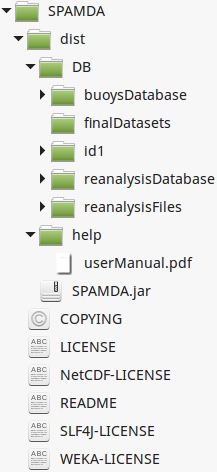
\includegraphics[scale=0.40]{figures/installationOnLinux.png}
					\caption{Content of the folder after installing SPAMDA (Linux).}
					\label{fig:installationOnLinux}
				\end{figure}
				
				Following, the structures of each folder and file created as a result of the installation are described:
				
					\begin{itemize}
						\item \textbf{\textit{dist}}: Contains the binary distribution of SPAMDA, which consist of:
							\begin{itemize}
								\item \textbf{\textit{DB}}: Contains all the information managed by SPAMDA.
									\begin{itemize}
										\item \textbf{\textit{buoysDatabase}}: Contains the database of the buoys.
										\item \textbf{\textit{finalDatasets}}: It is used as a default folder to save the final datasets.
										\item \textbf{\textit{id1}}: Contains the information of the buoy (annual text files, intermediate datasets, pre-processed datasets and matching configurations) entered as example.
										\item \textbf{\textit{reanalysisDatabase}}: Contains the database of the reanalysis data.
										\item \textbf{\textit{reanalysisFiles}}: Contains the reanalysis files entered through SPAMDA.
									\end{itemize}
								\item \textbf{\textit{help}}: Contains the user manual of SPAMDA.
									\begin{itemize}
										\item \textbf{\textit{userManual.pdf}}: This is the user manual.
									\end{itemize}
								\item \textbf{\textit{SPAMDA.jar}}: This is the runnable file containing SPAMDA.
							\end{itemize}
						\item \textbf{\textit{COPYING}}: This file contains a copy of the license of the GNU GENERAL PUBLIC LICENSE.
						\item \textbf{\textit{LICENSE}}: This file contains a copy of the license of SPAMDA.
						\item \textbf{\textit{NetCDF-LICENSE}}: This file contains a copy of the license of the Library NetCDF Java version 4.6.10
						\item \textbf{\textit{README}}: This file contains the instructions for getting started with SPAMDA.
						\item \textbf{\textit{SLF4j-LICENSE}}: This file contains a copy of the license of the Library SLF4J version 1.7.25
						\item \textbf{\textit{WEKA-LICENSE}}: This file contains a copy of the license of the Library WEKA version 3.8.1
					\end{itemize}
				
				After installing SPAMDA, and in order to run it, open the ``dist'' folder (as shown in Fig. \ref{fig:runningSPAMDAonLinux}) and type the following command on the command-line of the terminal:
				
				\texttt{java -jar SPAMDA.jar}
				
				\begin{figure}[ht!]
					\centering
					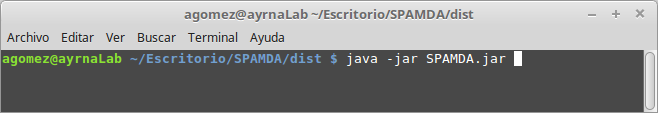
\includegraphics[scale=0.50]{figures/runningSPAMDAonLinux.png}
					\caption{Running SPAMDA on Linux.}
					\label{fig:runningSPAMDAonLinux}
				\end{figure}
				
				After executing such command, the main view of SPAMDA represented in Figure \ref{fig:SPAMDAmainViewonLinux} will appear.
				
				\begin{figure}[ht!]
					\centering
					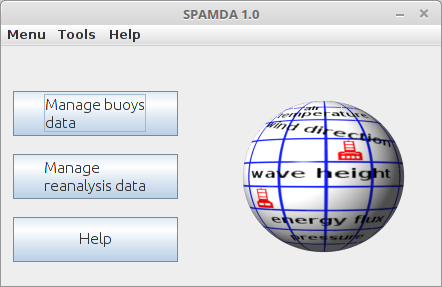
\includegraphics[scale=0.50]{figures/mainView.png}
					\caption{SPAMDA main view (Linux).}
					\label{fig:SPAMDAmainViewonLinux}
				\end{figure}

				
			\subsection{Installing on Windows}
			
				To install SPAMDA on Windows follow the next steps:
			
					\begin{itemize}
						\item \textit{\textbf{Step 1}}: Download the SPAMDA software on the computer.
						\item \textit{\textbf{Step 2}}: Create a folder and copy the downloaded file inside it.
						\item \textit{\textbf{Step 3}}: Decompress the file.
					\end{itemize}
					
				After performing the above steps SPAMDA would be installed on the computer and ready to be run. Note that the process of installation creates all the folders and files necessary inside the folder created in \textit{\textbf{Step 2}}. In Fig. \ref{fig:installationOnWindows} is represented an example of installation in the folder named ``SPAMDA'', which will contain the software tool.
				
				\begin{figure}[ht!]
					\centering
					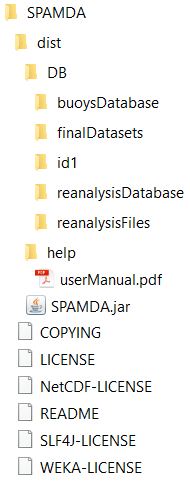
\includegraphics[scale=0.60]{figures/installationOnWindows.png}
					\caption{Content of the folder after installing SPAMDA (Windows).}
					\label{fig:installationOnWindows}
				\end{figure}
				
				Following, the structures of each folder and file created as a result of the installation are described:
				
					\begin{itemize}
						\item \textbf{\textit{dist}}: Contains the binary distribution of SPAMDA, which consist of:
							\begin{itemize}
								\item \textbf{\textit{DB}}: Contains all the information managed by SPAMDA.
									\begin{itemize}
										\item \textbf{\textit{buoysDatabase}}: Contains the database of the buoys.
										\item \textbf{\textit{finalDatasets}}: It is used as a default folder to save the final datasets.
										\item \textbf{\textit{id1}}: Contains the information of the buoy (annual text files, intermediate datasets, pre-processed datasets and matching configurations) entered as example.
										\item \textbf{\textit{reanalysisDatabase}}: Contains the database of the reanalysis data.
										\item \textbf{\textit{reanalysisFiles}}: Contains the reanalysis files entered through SPAMDA.
									\end{itemize}
								\item \textbf{\textit{help}}: Contains the user manual of SPAMDA.
									\begin{itemize}
										\item \textbf{\textit{userManual.pdf}}: This is the user manual.
									\end{itemize}
								\item \textbf{\textit{SPAMDA.jar}}: This is the runnable file containing SPAMDA.
							\end{itemize}
						\item \textbf{\textit{COPYING}}: This file contains a copy of the license of the GNU GENERAL PUBLIC LICENSE.
						\item \textbf{\textit{LICENSE}}: This file contains a copy of the license of SPAMDA.
						\item \textbf{\textit{NetCDF-LICENSE}}: This file contains a copy of the license of the Library NetCDF Java version 4.6.10
						\item \textbf{\textit{README}}: This file contains the instructions for getting started with SPAMDA.
						\item \textbf{\textit{SLF4j-LICENSE}}: This file contains a copy of the license of the Library SLF4J version 1.7.25
						\item \textbf{\textit{WEKA-LICENSE}}: This file contains a copy of the license of the Library WEKA version 3.8.1
					\end{itemize}
				
				After installing the software, and in order to run it, open the ``dist'' folder and double-click on the SPAMDA.jar file. Next, the main view of SPAMDA represented in figure \ref{fig:SPAMDAmainViewonWindows} will appear.
				
				\begin{figure}[ht!]
					\centering
					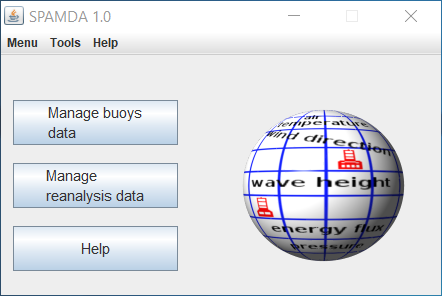
\includegraphics[scale=0.80]{figures/mainViewonWindows.png}
					\caption{SPAMDA main view (Windows).}
					\label{fig:SPAMDAmainViewonWindows}
				\end{figure}

			
			\subsection{Installing on macOS}
			
				To install SPAMDA on macOS follow the next steps:
			
					\begin{itemize}
						\item \textit{\textbf{Step 1}}: Download the SPAMDA software on the computer.
						\item \textit{\textbf{Step 2}}: Create a folder and copy the downloaded file inside it.
						\item \textit{\textbf{Step 3}}: Decompress the file.
					\end{itemize}
					
				After performing the above steps SPAMDA would be installed on the computer and ready to be run. Note that the process of installation creates all the folders and files necessary inside the folder created in \textit{\textbf{Step 2}}. In Fig. \ref{fig:installationOnMacOS} is represented an example of installation in the folder named ``SPAMDA'', which will contain the software tool.
				
				\begin{figure}[ht!]
					\centering
					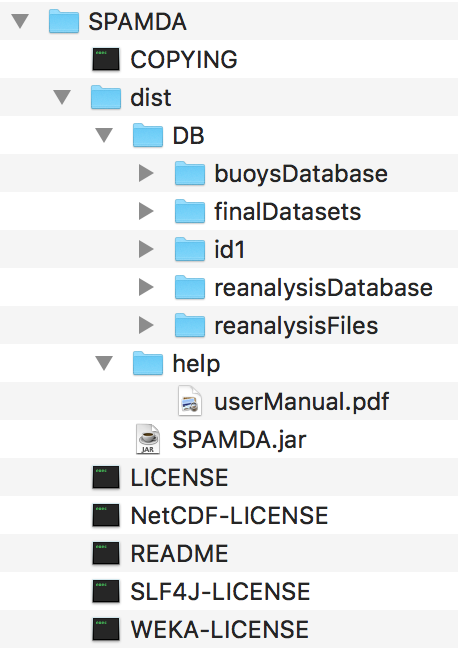
\includegraphics[scale=0.60]{figures/installationOnMacOS.png}
					\caption{Content of the folder after installing SPAMDA (macOS).}
					\label{fig:installationOnMacOS}
				\end{figure}
				
				Following, the structures of each folder and file created as a result of the installation are described:
				
					\begin{itemize}
						\item \textbf{\textit{dist}}: Contains the binary distribution of SPAMDA, which consist of:
							\begin{itemize}
								\item \textbf{\textit{DB}}: Contains all the information managed by SPAMDA.
									\begin{itemize}
										\item \textbf{\textit{buoysDatabase}}: Contains the database of the buoys.
										\item \textbf{\textit{finalDatasets}}: It is used as a default folder to save the final datasets.
										\item \textbf{\textit{id1}}: Contains the information of the buoy (annual text files, intermediate datasets, pre-processed datasets and matching configurations) entered as example.
										\item \textbf{\textit{reanalysisDatabase}}: Contains the database of the reanalysis data.
										\item \textbf{\textit{reanalysisFiles}}: Contains the reanalysis files entered through SPAMDA.
									\end{itemize}
								\item \textbf{\textit{help}}: Contains the user manual of SPAMDA.
									\begin{itemize}
										\item \textbf{\textit{userManual.pdf}}: This is the user manual.
									\end{itemize}
								\item \textbf{\textit{SPAMDA.jar}}: This is the runnable file containing SPAMDA.
							\end{itemize}
						\item \textbf{\textit{COPYING}}: This file contains a copy of the license of the GNU GENERAL PUBLIC LICENSE.
						\item \textbf{\textit{LICENSE}}: This file contains a copy of the license of SPAMDA.
						\item \textbf{\textit{NetCDF-LICENSE}}: This file contains a copy of the license of the Library NetCDF Java version 4.6.10
						\item \textbf{\textit{README}}: This file contains the instructions for getting started with SPAMDA.
						\item \textbf{\textit{SLF4j-LICENSE}}: This file contains a copy of the license of the Library SLF4J version 1.7.25
						\item \textbf{\textit{WEKA-LICENSE}}: This file contains a copy of the license of the Library WEKA version 3.8.1
					\end{itemize}
				
				After installing the software, and in order to run it, open the ``dist'' folder and double-click on the SPAMDA.jar file. Next, the main view of SPAMDA represented in figure \ref{fig:SPAMDAmainViewonMacOS} will appear.
				
				\begin{figure}[ht!]
					\centering
					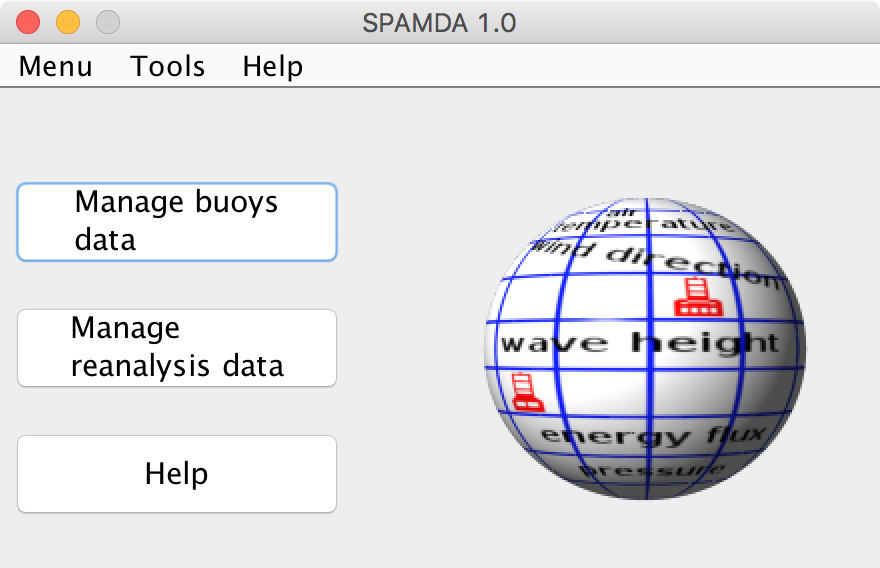
\includegraphics[scale=0.50]{figures/mainViewonMacOS.png}
					\caption{SPAMDA main view (macOS).}
					\label{fig:SPAMDAmainViewonMacOS}
				\end{figure}

			
		\section{How to uninstall?}
		
			To uninstall SPAMDA just delete the folder in which the installation process was carried out. 
			
			\begin{center}
				\begin{warningbox}{Warning}{13cm}
					This action will remove SPAMDA from your computer and any information entered in SPAMDA or generated by means of it will be lost.
				\end{warningbox}
			\end{center}

	\end{onehalfspace}
